\clearpage
\thispagestyle{empty}
\addcontentsline{toc}{chapter}{\hspace{6mm}\textbf{CHAPTER 4 \hspace{8mm} RESULTS AND DISCUSSION \hspace{4.9cm}}}

\begin{center}
	\textbf{{CHAPTER 4}}\\
	\vspace{-1ex}
	\textbf{RESULTS AND DISCUSSION}
	\vspace{-3ex}
\end{center}

This chapter presents the results and analysis of findings made in the conduct of the study. (Objective #1) This includes discussion of the developed Topic Modelling Tool that can collect, pre-process and generates topic models. (Objective #2) The Latent Dirichlet Allocation algorithm used to generate topic models, and (Objective #3) the extent of correctness of the generated topic models based on its topic coherence.  

\subsection{Features of the Develop NLP Tool / Game / Application}
\vspace{-2ex}
{\textbf{Uploading of Data.}}  Data can be uploaded in the main interface window where the upload tab is located as shown in the figure below. The system accepts .txt data file as well as multiple .txt files placed in a folder. It follows mallet syntax for importing documents, import-dir command for multiple .txt files and import-file command for individual .txt file. \\
\vspace{-1ex}
	
    \begin{figure}[H]
            \centering
            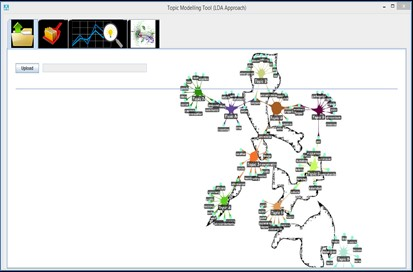
\includegraphics[width=15cm,height=9cm]{image/cs_figure1.jpg}
            \caption{Main Interface with the Upload Tab Window}
	\end{figure}
	
\textbf{Pre-processing of Data. }In the clean data tab shown in figure 2, the system included the default English Mallet stopwords to be deleted form the uploaded dataset. It allows user to view the default Mallet English stopwords, upload additional stopwords in .txt files, as well as create a new stoplist. Users can also add word or words that will automatically be added to the existing uploaded or created stoplists. 

Lastly, from the uploaded, created or added words in the list, users can also delete word or words by highlighting or selecting them. These cleaning options can assure that the topic model to be generated will be more appropriate.

    \begin{figure}[H]
	\centering
	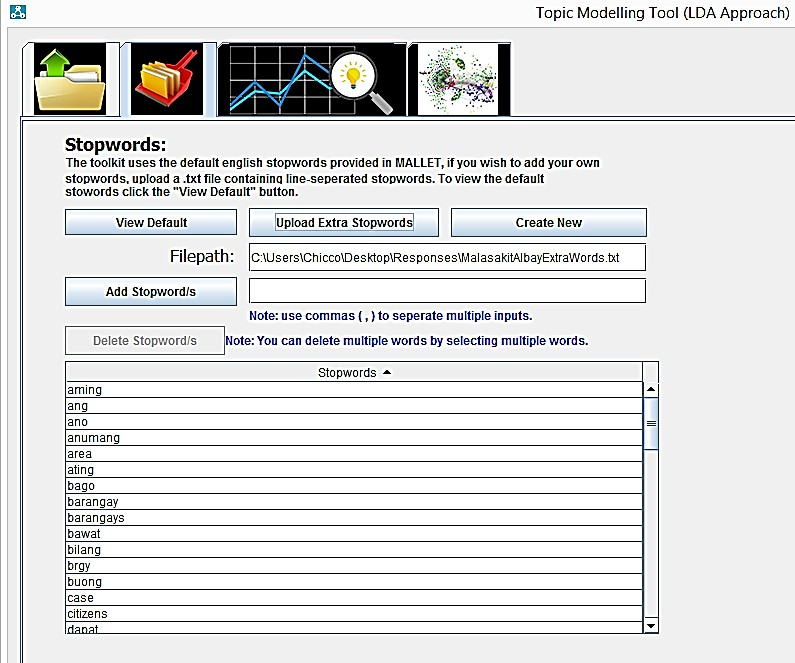
\includegraphics[width=13cm,height=7cm]{image/cs_figure2.jpg}
	\caption{Stopwords Options}
	\end{figure}

\textbf{Processing of Data.} Processing of the cleaned data sets starts with the click of the run button, the system then displays the required parameters in order for it to generate a topic model. The following parameters as shown in figure 3 are required to generate a topic model. Number of topic indicates the number of topic models the user wants to generate. Number of iterations normally starts from 50 to 500, up-to 10,000. Iteration depends on the size of the data sets.

The smaller the datasets, low iteration should be sensible. The number of words indicates the words per topic, optimization interval assigns the occurrence value based on the Latent Dirichlet Allocation (LDA), and the model name is the created file of the generated topic model. Clicking the start button will begin the processing to generate topic model with the given parameters. 

    \begin{figure}[H]
	\centering
	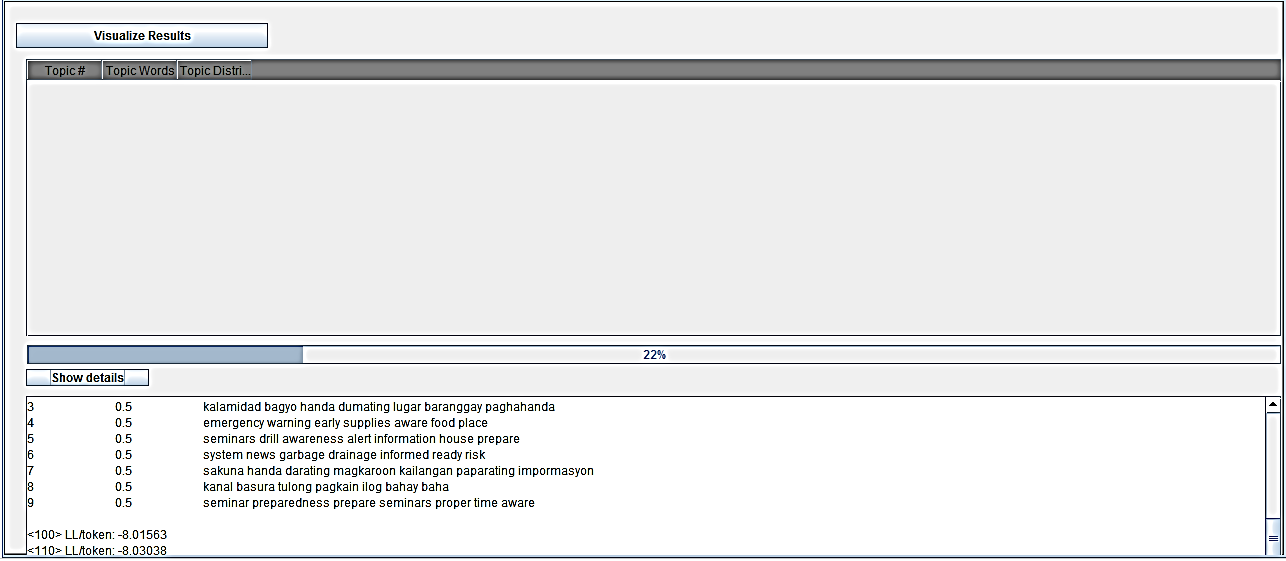
\includegraphics[width=13cm,height=7cm]{image/cs_figure3.png}
	\caption{Processing for Topic Modeling}
	\end{figure}

\textbf{Game Modes.} The Segregation Game is a 2D swipe-and-shoot game developed for android in order to teach the users how waste segregation is properly done. The game has two modes, the Player vs. A.I. mode in which the player will play against an A.I. opponent in easy, medium or hard difficulty, and the Player vs. Player mode in which the player will play against another player in a local area network or WLAN.

    \begin{figure}[H]
	\centering
	
\includegraphics[width=4cm,height=7cm]{image/cs_figure4_1.jpg}
	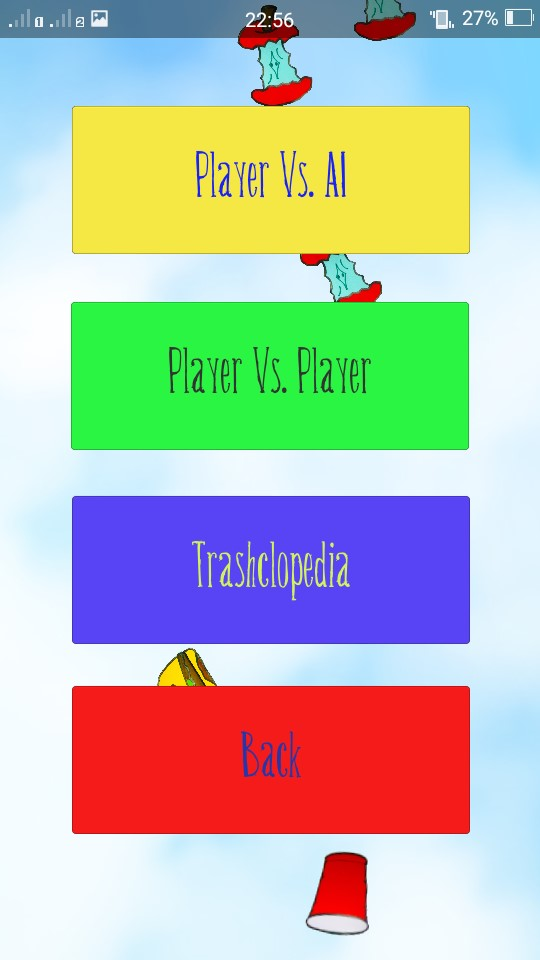
\includegraphics[width=4cm,height=7cm]{image/cs_figure4_2.jpg}
	\caption{The Segregation Game’s Main Menu and Game Modes}
	\end{figure}

\textbf{Difficulty Levels.} There are three difficulty levels in the game, the “easy” difficulty in which the opponent taps the screen in a slow pace (3 seconds), the “normal” difficulty in which the A.I. taps the screen in a faster pace (1.5 seconds) and the “hard” difficulty in which the A.I. taps the screen in the fastest pace (1 second).

\textbf{The “Trashclopedia”.} The “Trashclopedia” has three parts as seen in figure 5, the “Trash Talk”, the definition of terms regarding waste segregation, the “Trivia” has useful facts for the user’s knowledge and enjoyment, and the “Classification”, the classification of the in-game objects that are classified into biodegradable and non-biodegradable. 

    \begin{figure}[H]
	\centering
	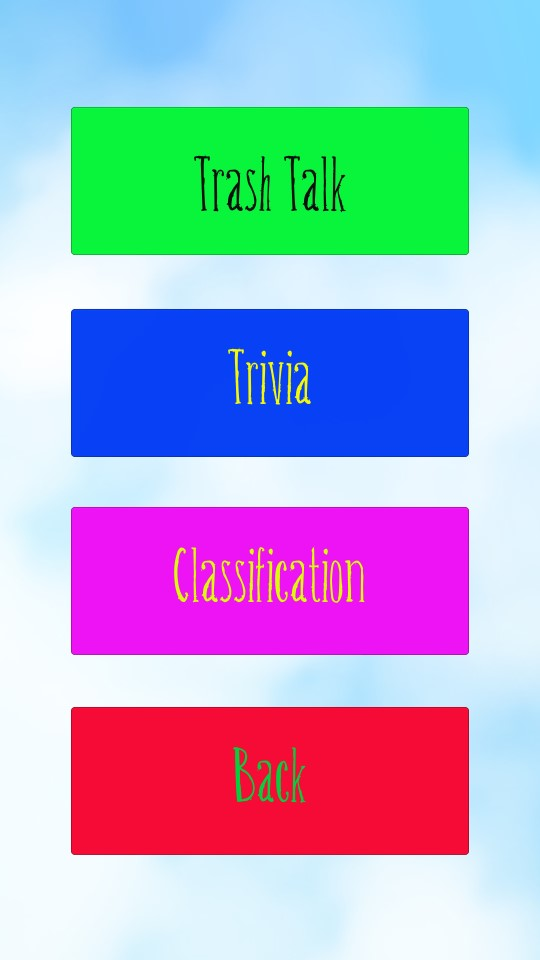
\includegraphics[width=4cm,height=7cm]{image/cs_figure5.jpg}
	\caption{The Trashclopedia}
	\end{figure}

\textbf{Latent Dirichlet Allocation (LDA) Algorithm used to appropriately categorize similar groups of data.}  In natural language processing, is a generative model that allows sets of observations to be explained by unobserved groups that explain why some parts of the data are similar. Using a plate notation to represent the Latent Dirichlet Allocation (LDA) approach, the dependencies among the many variables can be captured concisely. Figure 6 represents the following: The boxes are “plates” representing replicates; the outer plate represents documents, while the inner plate represents the repeated choice of topics and words within a document. M denotes the number of documents, N the number of words in a document.

    \begin{figure}[H]
	\centering
	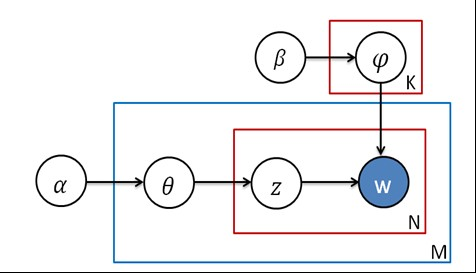
\includegraphics[width=12cm,height=7cm]{image/cs_figure6.jpg}
	\caption{Plate notation for LDA with Dirichlet-distributed topic-word}
	\end{figure}

\noindent Where:
\vspace{-2ex}
\begin{enumerate}
	\item [] α (alpha) is the parameter of the Dirichlet prior on the per-document topic distributions;
	\item [] β (beta) is the parameter of the Dirichlet prior on the per-topic word distribution;
	\item [] θ(theta)M  is the topic distribution for document M;
	\item [] φ(phi)K is the word distribution for topic K;
	\item [] Zmn is the topic for the n-th word in document M; and
	\item [] Wmn is the specific word.
\end{enumerate}

\subsection{Algorithm used for the Developed System / Application to achieve the necessary functions or output/s of the study.}

Latent Dirichlet Allocation (LDA) assumes documents are produced from a mixture of topics, these topics then generate words based on their probability distribution. Given a dataset of documents, LDA backtracks and tries to figure out what topics would create those documents. LDA is a matrix factorization technique. In vector space, any corpus can be represented as a document-term matrix.

\textbf{Parameters of Latent Dirichlet Allocaton (LDA).} Parameters are vital in the correctness of the generation of models in topic modeling. The following are the LDA parameters:

Alpha and Beta. Alpha and Beta hyper-parameters are the key parameters of LDA where alpha represents document-topic density and Beta represents topic-word density. Higher the value of alpha, documents are composed of more topics and lower the value of alpha, documents contain fewer topics. On the other hand, higher the beta, topics are composed of a large number of words in the corpus, and with the lower value of beta, they are composed of few words.

Number of Topics. These are the number of topics to be extracted from the corpus. Researchers have developed approaches to obtain an optimal number of topics by using Kullback Leibler Divergence Score.

Number of Topic Terms. The number of terms composed in a single topic where generally is determined according to the requirement. If the problem statement talks about extracting themes or concepts, it is recommended to choose a higher number, if problem statement talks about extracting features or terms, a low number is recommended.

Number of Iterations / passes. The maximum number of iterations allowed to LDA algorithm for convergence.
	
\textbf{Djikstra’s algorithm to compute the distances between nodes.} The Djikstra’s algorithm computes the distances between nodes as shown in figure 7. It gets the values of the designated paths and it computes the distances between the indexes which are represented as nodes in the map. The researchers plotted the nodes in each path through the x and y coordinates of the image. The nodes are called in the algorithm to determine the point of origin and the destination and to display the paths.

    \begin{figure}[H]
	\centering
	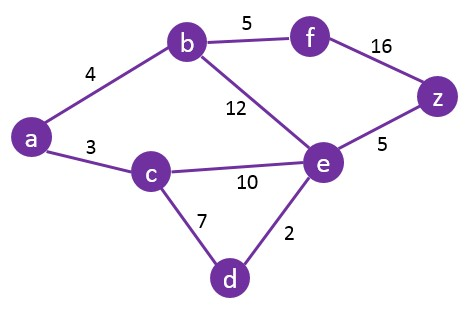
\includegraphics[width=12cm,height=7cm]{image/cs_figure7.jpg}
	\caption{Shortest Path using Djiktra Algorithm}
	\end{figure}

\textbf{Application of Recurrent Neural Network Algorithm in Disaster Management.} Recurrent neural network, shown in figure 8 is a type of ANN, where it takes input not just the current example they see, but also what they have perceived previously in time.  It has recurrent means of interpreting and assessing the current information being processed. RNN can utilize distributed representations of words by first converting the tokens comprising each text into vectors, which form a matrix. Networks main advantage resides in their ability to deal with sequential data. The prediction by the network at time-step T is influenced by the one it made at time-step T – 1.This chapter presents the results and analysis of findings made in the conduct of the study. (Objective #1) This includes discussion of the developed Topic Modelling Tool that can collect, pre-process and generates topic models. (Objective #2) The Latent Dirichlet Allocation algorithm used to generate topic models, and (Objective #3) the extent of correctness of the generated topic models based on its topic coherence.  

    \begin{figure}[H]
	\centering
	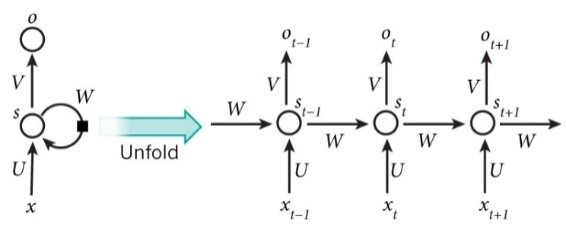
\includegraphics[width=12cm,height=6cm]{image/cs_figure8.jpg}
	\caption{Recurrent Neural Network}
	\end{figure}

%--------------------------------------------------------------------------------------------
\textbf{Extent of correctness of the generated topic models based on its topic coherence}

\textbf{Evaluating the Topic Models through Human Judgment.} The generated topic models can be measured by evaluating the performance of the Latent Dirichlet Allocation (LDA). Evaluating the LDA can be done using human judgments to examine the topics. This may involve identifying semantic coherent topics and measuring if topic model’s association agrees with human topic associations for a dataset. 

One method of measuring its correctness is by comparing the directly annotated topic assignments based on its top-N words and validate if these annotations agree with the human judgment. 

\textbf{Model Precision.} Model precision was used to measure the correctness of the generated topic model against manually annotated models. It is the number of agreements between humans and the model divided by the total number of judgments. Table 1 presents the results to measure the correctness of the generated topic model against the manually annotated ones. Test 1 returned 100\% precision, test 2 with 83\% precision and test 3 returned an 85\% precision. 
In summary, the average precision rated 87\% denoting that the manual annotations of the generated topic models agreed with the human judgments. The respondents view on the topics marked with “No Label” disagreed to their judgment implying that there could be themes assigned. These were true enough because finding shows that the topics have coherent aspects but words were evenly distributed indicating possible assignments of multiple labels.



\begin{table}[H]
	\centering
	\caption{Precision Results}
	\centering
	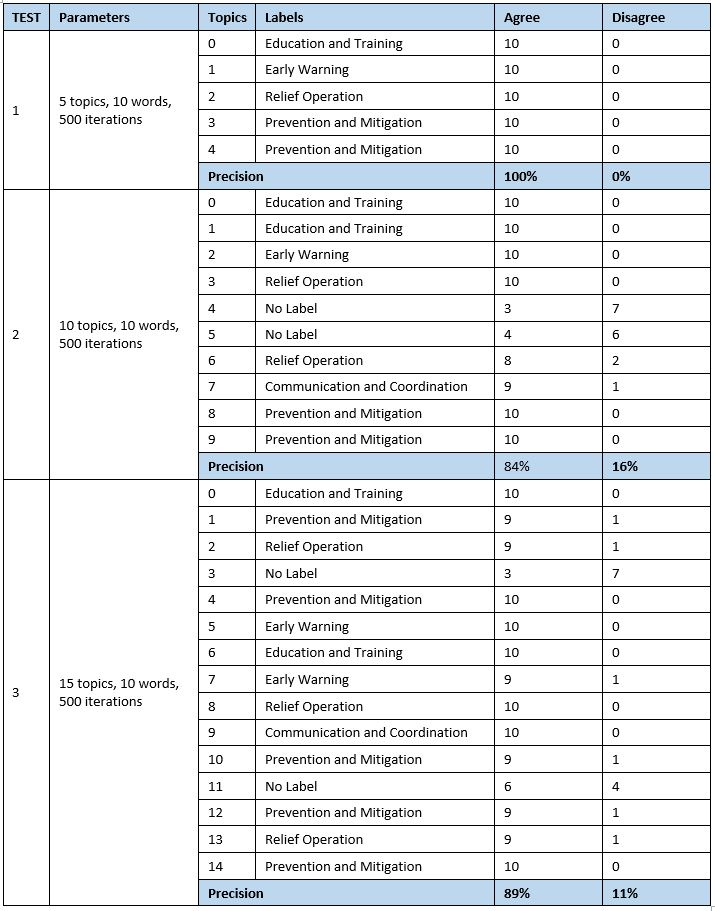
\includegraphics[width=12cm,height=16cm]{image/cs_table1.jpg}
\end{table}

\subsection{Performance Evaluation of the Classification Models using accuracy, precision F measures and recall metrics. }

\textbf{Performance Evaluation.} Performance of the classification models were described by the confusion matrices which were used to properly present the classified data. The classifier configuration that obtained the best accuracy was selected to be used in developing the DRM e-Participatory toolkit qualitative response classification system. The average accuracy, precision, recall were computed to give overall assessment of the effectiveness of the classification across the defined categories for the DRM qualitative responses.

Accuracy measured the effectiveness of the classifier in terms of detections in agreement with the actual classifications.  Formula 1 shows the formula on determining the accuracy of the model.

%Formula 1
\begin{center}
Formula 1. \textit{ Accuracy}
\end{center}
\vspace{-2ex}
\begin{equation}
\begin{align*}
Accuracy &= \frac{No. of Correctly Classified Responses}{Total no.of Qualitative Responses}\
\end{align*}
\end{equation}
%Formula 1

On the other hand, precision measured the exactness of a classifier and considers false detection. A higher precision means less false positives, while a lower precision means more false positives. Formula 2 shows how precision is computed.

%Formula 2
\begin{center}
Formula 2. \textit{Precision}
\end{center}
\begin{equation}
\begin{align*}
Precision &= \frac{True Positives}{True positives + False positives}\
\end{align*}
\end{equation}

%Formula 2

Recall measures the completeness, or sensitivity, of the classifier. Higher recall means less false negatives, while lower recall means more false negatives.

%Formula 3
\begin{center}
Formula 3. \textit{Recall}
\end{center}
\begin{equation}
\begin{align*}
Recall &= \frac{True Positives}{True positives+False negatives}\
\end{align*}
\end{equation}
%Formula 3


The last metric, which is F-measure is computed using the formula shown below. It is the weighted harmonic mean of precision and recall and its main advantage is it is able to rate a system with one unique rating. 

%Formula 4
\begin{center}
Formula 4. \textit{F-measure}
\end{center}
\begin{equation}
\begin{align*}
F - measure &= \frac{2*precision*recall}{precision + recall}\
\end{align*}
\end{equation}
%Formula 3

\textbf{Results of Experiments.} The performance of the classification models were determined by the standard metrics discussed in the previous section. Metric scores of regular and bidirectional neural networks are shown in table 2. It is observed that the two RNN algorithms produced closed evaluation results where Bidirectional RNN obtained accuracy rate of  81.67\%, 81.17 precision, 81.67\% recall and 80.81\% f-measure against performance evaluation result of regular RNN where is obtained 81.25\% accuracy, 80.84\% precision, 81.25\% recall and 80.25\% f-measure.

\begin{table}[H]
	\centering
	\caption{Summary of Precision Results}
	\begin{tabular}{ | C{3cm}| C{3cm} | C{3.5cm} |}
	\hline
	\textbf{Standard Metric} & \textbf{Regular RNN} & \textbf{Bidirectional RNN}\\
	\hline 
	\textbf{Accuracy} & 81.25\% & \textbf{81.67\%}\\
	\hline
	\textbf{Precision} & 80.84\% & \textbf{81.17\%}\\
	\hline
	\textbf{Recall} & 81.25\% & \textbf{81.67\%}\\
	\hline
	\textbf{F-measure} & 80.25\% & \textbf{80.81\%}\\
	\hline
	\end{tabular}
\end{table}


